\documentclass[10pt]{extarticle}
\usepackage[sfdefault]{FiraSans}
\usepackage[T1]{fontenc}
\usepackage[utf8]{inputenc}
\usepackage{adjustbox}
\usepackage{algorithm}
\usepackage{algorithmic}
\usepackage{amsfonts}
\usepackage{amsmath}
\usepackage{amssymb}
\usepackage[style=apa]{biblatex}
\addbibresource{references.bib}
\usepackage{booktabs}
\usepackage{breqn}
\usepackage{enumitem}
\usepackage{float}
\usepackage{geometry}
\usepackage{graphicx}
\usepackage{hyperref}
\usepackage{lipsum}
\usepackage{longtable}
\usepackage{multirow}
\usepackage{pdfpages}
\usepackage{pgfgantt}
\usepackage{setspace}
\usepackage{subcaption}
\usepackage{tabularx}
\usepackage{tikz}
\usepackage{xcolor}

\DeclareLanguageMapping{english}{english-apa}

\geometry{letterpaper, left=1in, right=1in, top=1in, bottom=1in,}

\definecolor{primary}{RGB}{0,120,215}
\definecolor{secondary}{RGB}{255,87,34}
\definecolor{background}{RGB}{245,245,245}
\definecolor{blue}{RGB}{0,62,126}

\pagecolor{background}

\hypersetup{colorlinks=true, linkcolor=primary, filecolor=secondary, urlcolor=primary, citecolor=black}

\AtBeginBibliography{\hypersetup{urlcolor=black}}

\setstretch{1.15}

\setlength{\bibhang}{0.5in}
\setlength\bibitemsep{1.5\itemsep}

\setlength{\parindent}{0pt}
\setlength{\parskip}{1em}

\nocite{*}

\begin{document}

\newcommand{\mytitlepage}[2]{
    \thispagestyle{empty}

    \begin{tikzpicture}[remember picture, overlay]
        \node [inner sep=0pt] at (current page.center) {#1}; { \node [ anchor=center, inner sep=1.25cm, rectangle, fill=blue!70!white, fill opacity=0, text opacity=1, minimum height=0.2\paperheight, minimum width=\paperwidth, text width=0.8\paperwidth, font=\fontfamily{pnc}\selectfont ] at (current page.center) {#2}; } \node [anchor=south east, outer sep=3pt] at (current page.south east) {\includegraphics[width=0.33\paperwidth]{logo.png}};
    \end{tikzpicture}

    \newpage
}

{ \mytitlepage{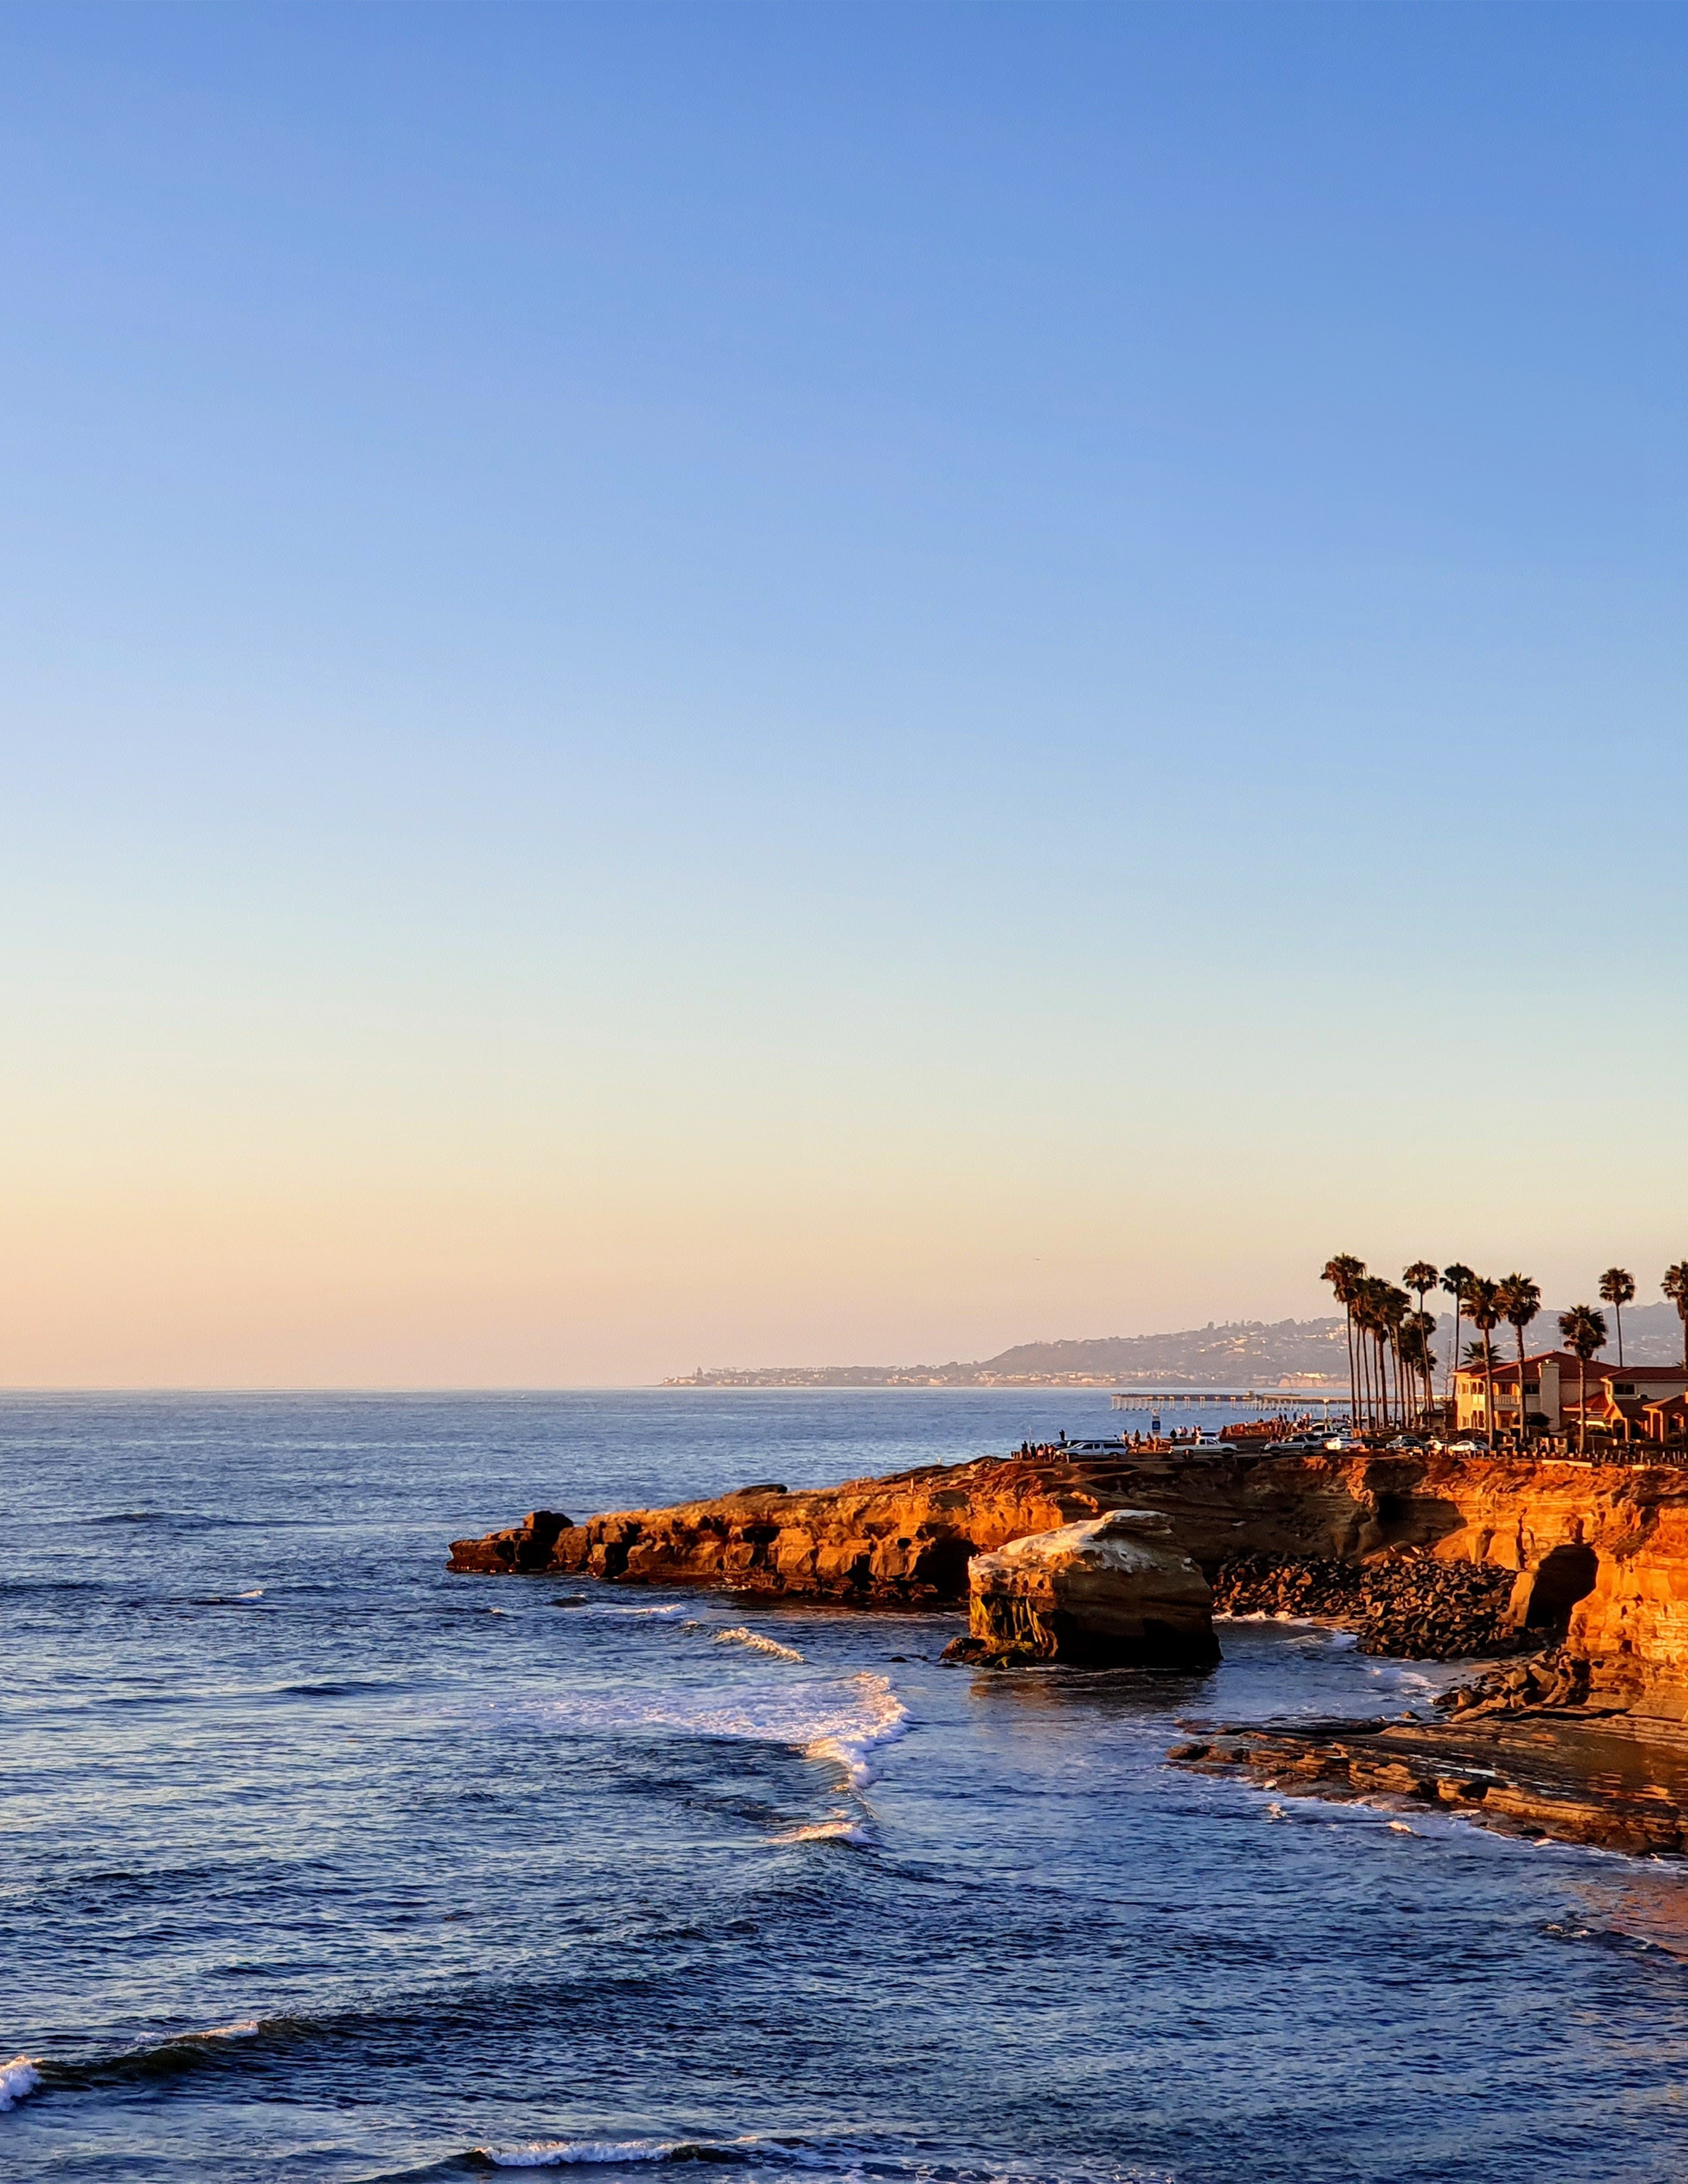
\includegraphics[width=\paperwidth]{background.png}}
    {
        \centering
        \fontfamily{phv}
        \vspace{-200pt} % move title up
        { \Huge
            \bfseries

            \begin{center}
                Next-Generation Health Monitoring: \\
                A Real-Time Approach to Fitness Tracking
            \end{center}

            \par
        }
        \vspace{8pt}
        { \Large
            \bfseries

            Final Project Progress Update

            \par
        }
        \vspace{24pt}
        {
            \begin{center}
                \begin{tabular*} {\textwidth}{@{\extracolsep{\fill}}c c c}
                    {\LARGE Jonathan Agustin} & {\LARGE Alec Anderson} & {\LARGE Brandon Smith}
                \end{tabular*}
            \end{center}
        }
    }
}

\pagenumbering{arabic}

\begin{center}
    {\LARGE \textbf{Next-Generation Health Monitoring:}} \\
    {\large \textbf{A Real-Time Approach to Fitness Tracking}}
\end{center}


\section{IoT System Design}

The team has made progress in creating a system that integrates wearable technology, a mobile app, and a cloud-based analytics platform. The wearable device keeps track of health and fitness information, sending it to the cloud for deeper study and examination. The mobile app is the user interface that gives people advice based on their health measurements and preferences. Connecting everything was tricky because we had to ensure all the interfaces were consistent within all system components.

We used industry-standard communication protocols like MQTT and HTTPS to ensure our system components could talk to each other without any problems. These protocols helped us send data securely and efficiently between the wearable device, cloud platform, and mobile app. We set up the message broker to manage the information flow and ensure everything arrived. Our mobile app is the main way people interact with our system. We wanted to create an easy-to-use design that provides helpful advice and tips based on their health data.

\section{Dataset Exploration and Cleaning}

When it came to preparing the data, we relied heavily on the PMData set, which needed a lot of cleaning and organizing. We discovered some issues with timestamps and missing health information. To fix these problems, we created a cleaning process that included fixing the timestamps and filling in the missing data. This made our dataset much better and ready for more analysis and training of our machine-learning models. The large amount of data caused issues with how fast our system could work and how much memory it used. So, we adjusted our data handling methods and used smarter storage techniques to make things run more smoothly.

\section{Deep Learning Machine Learning Method}

We use a Convolutional Neural Network (CNN) for deep learning. The CNN model helps us examine time-series data from the heart rate sensor to find patterns that might indicate hidden health issues, like arrhythmia or irregular beat intervals. Since CNNs are good at finding patterns in data that change over time, they are a great choice for analyzing this sequential data with important time-based features.

\section{Time Series Machine Learning Method}

In addition to the CNN, we use a Long Short-Term Memory (LSTM) model to meet the time-series prediction requirement. The LSTM model predicts future trends in heart rates based on past data. By looking at historical information, the LSTM can spot subtle changes that might indicate potential problems, such as stress, overexertion, or other health concerns. Since LSTMs can store important information over long periods, they are great for time-series forecasting based on past observations.

\newpage

\printbibliography

\newpage

\end{document}
